\documentclass[11pt]{report}

\usepackage[left=0.75in, right=0.75in, top=0.75in, bottom=0.75in]{geometry}
\setlength\parindent{0pt}

\usepackage{graphicx, amsmath,anonchap,tabularx,multicol}
\usepackage{wasysym}

\usepackage{enumitem}
\setlist{noitemsep}
\setlist{nolistsep}


%%%
% Set up some shortcut commands
%%%
\newcommand{\R}{\mathbb{R}}
\newcommand{\N}{\mathbb{N}}
\newcommand{\Z}{\mathbb{Z}}
\newcommand{\Proj}{\mathrm{proj}}
\newcommand{\Perp}{\mathrm{perp}}
\newcommand{\proj}{\mathrm{proj}}
\newcommand{\Span}{\mathrm{span}}
\newcommand{\Null}{\mathrm{null}}
\newcommand{\Rank}{\mathrm{rank}}
\newcommand{\mat}[1]{\begin{bmatrix}#1\end{bmatrix}}



\begin{document}
\pagestyle{empty}

\begin{center}{\Large{\textbf{Math 240: Peer-Assisted Reflection \#1}}}\end{center}

\begin{tabular*}{\textwidth}{@{\extracolsep{\fill}}l l}
\textbf{Due Dates: 9/29 (draft), 9/30 (final)}   & Name: \rule{6cm}{0.5pt} \\
\hline\hline
\end{tabular*} \\

\textbf{The PAR Process}

\begin{center}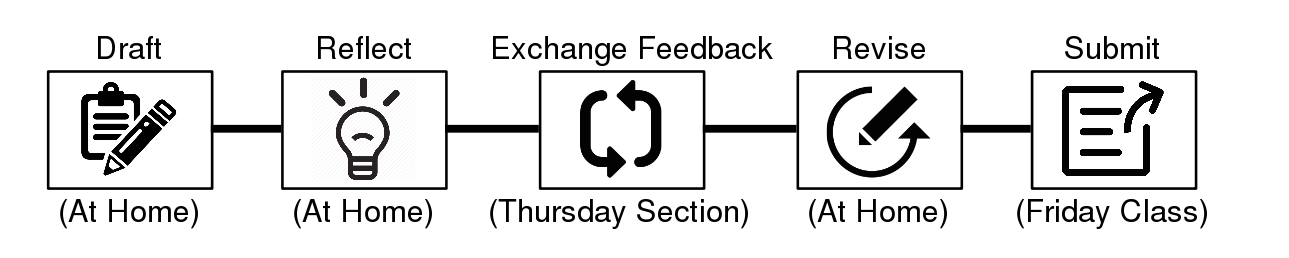
\includegraphics[scale=0.7]{flow_chart.pdf}\end{center}

\textit{Note: Write your draft on a separate sheet and bring it to section.  I will pass out a hard copy of this sheet for your self-reflection; bring that to section as well.  Turn in both on Friday, plus your final draft.}

\bigskip

\textbf{Problem Statement}


	The newly-appointed queen of a newly-discovered land hires three
	explorers to map her territory: Emily, Jack, and Lila.  The explorers
	have their own equipment and their own quirks.
	\begin{enumerate}
		\item[Jack] Jack has a miscalibrated compass---it is off by 45$^\circ$.
		When Jack thinks he's walking east, he is actually walking
		due northeast.  When Jack walks in what he thinks is a cardinal
		direction, he measures distance accurately.
		\item[Emily] Emily is a careful explorer with an accurate compass.
		When Emily measures distance in a cardinal direction, it too
		is accurate.
		\item[Lila] Lila is an excitable explorer.  Her compass is accurate, but when 
		she walks north, she skips and twirls.  As a consequence, when Lila
		walks north, the distance she thinks she travels is \emph{half} the distance she actually
		traveled.
	\end{enumerate}
	Further, each explorer only walks in what they think are cardinal directions (i.e., north, east,
	south, and west).  The queen declares that her palace is the center of the nation and that all
	measurements be made relative to her palace.  She then sends the explorers on their way.
	\begin{enumerate}
		\item Emily finds the ruins of an ancient civilization located 70 miles east and
		40 miles north of the queen's palace.  She records the \emph{royal coordinates}
		$(70,40)$ in her logbook.  The other explorers find the same ruins.  What
		coordinates do they record in their logbook?
		\item Each explorer is familiar with the Pythagorean theorem, and uses it with
		his/her own coordinates to compute
		the distance from the palace to the ruins.  What distances do they compute?
		Are they all the same?  Explain why any differences or similarities appear
		in the distance calculation.
		\item The queen values accuracy and will behead anyone who reports inaccurate distances
		(strangely, the queen is just fine with inaccurate directions).
		Lila, unfortunately, cannot be convinced to change her coordinates.  However,
		she might be convinced to use a different formula for distance, rather
		than the Pythagorean theorem.  Is there a formula that Lila can use
		to accurately compute distances from her coordinates?
		\item Suppose that Jack starts skipping and twirling and records a distance
		\emph{half} as far as he actually travels when he thinks he's walking
		north.  Is there a formula that he can use to compute distances accurately?
		How does this formula relate to Lila's?  Explain.
	\end{enumerate}



\vspace{0.5in}

\begin{center}{\Large{\textbf{Reflection\\}}}

Turn the page and check off the icons that you think you did well; circle icons that you want feedback on. \end{center}

\newpage

\begin{center}{\Large{\textbf{Feedback Provided By: \rule{6cm}{0.5pt}}}}\end{center}

\begin{tabular*}{\textwidth}{@{\extracolsep{\fill}}l c r}
\textbf{Suggestions} & Communication & \textbf{Strengths}  \\
\hline
\end{tabular*}
\begin{center}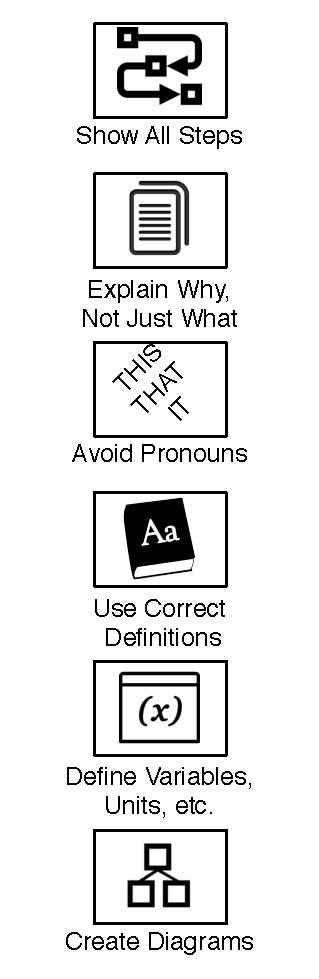
\includegraphics[scale=0.7]{communication.pdf}\end{center}

\begin{tabular*}{\textwidth}{@{\extracolsep{\fill}}l c r}
\textbf{Suggestions} & Accuracy & \textbf{Strengths}  \\
\hline
\end{tabular*}

\begin{center}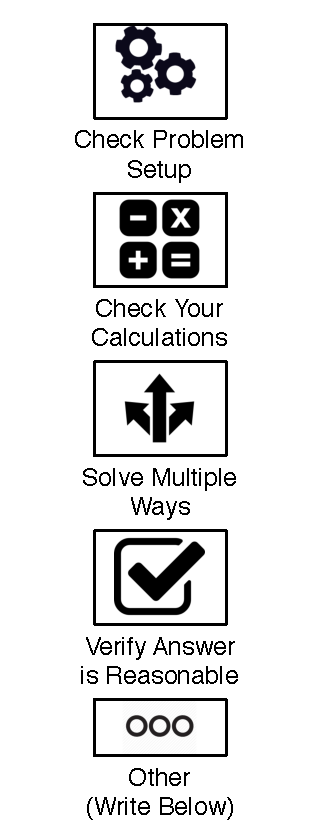
\includegraphics[scale=0.7]{accuracy.pdf}\end{center}




\end{document}
